\label{ch:appendix}

\section{Wind direction correction} \label{app:wind_dir}

Figure \ref{fig:csat3b_correction} shows the comparison between the wind direction of the CSAT3-B and the CSAT3 No.5, both separated by 30~cm. The blue points show the uncorrected data, where is possible to see that there is a linear relationship between both instruments, but it is inverted and has a constant phase separation. Because of these, we proposed as a correction 

$$\theta_{c} = (-\theta-90\degree) \mod 360,$$

\noindent where we took the inverse of the wind direction ($\theta$) and subtract it by $90\degree$. Module 360 is applied to preserve a value between [$0\degree$, $360\degree$]. As we can see from the orange points in the figure~\ref{fig:csat3b_correction}, the corrected data is totally correlated to the wind direction measured with the CSAT3 No.5.

\begin{figure}[!ht]
    \centering
    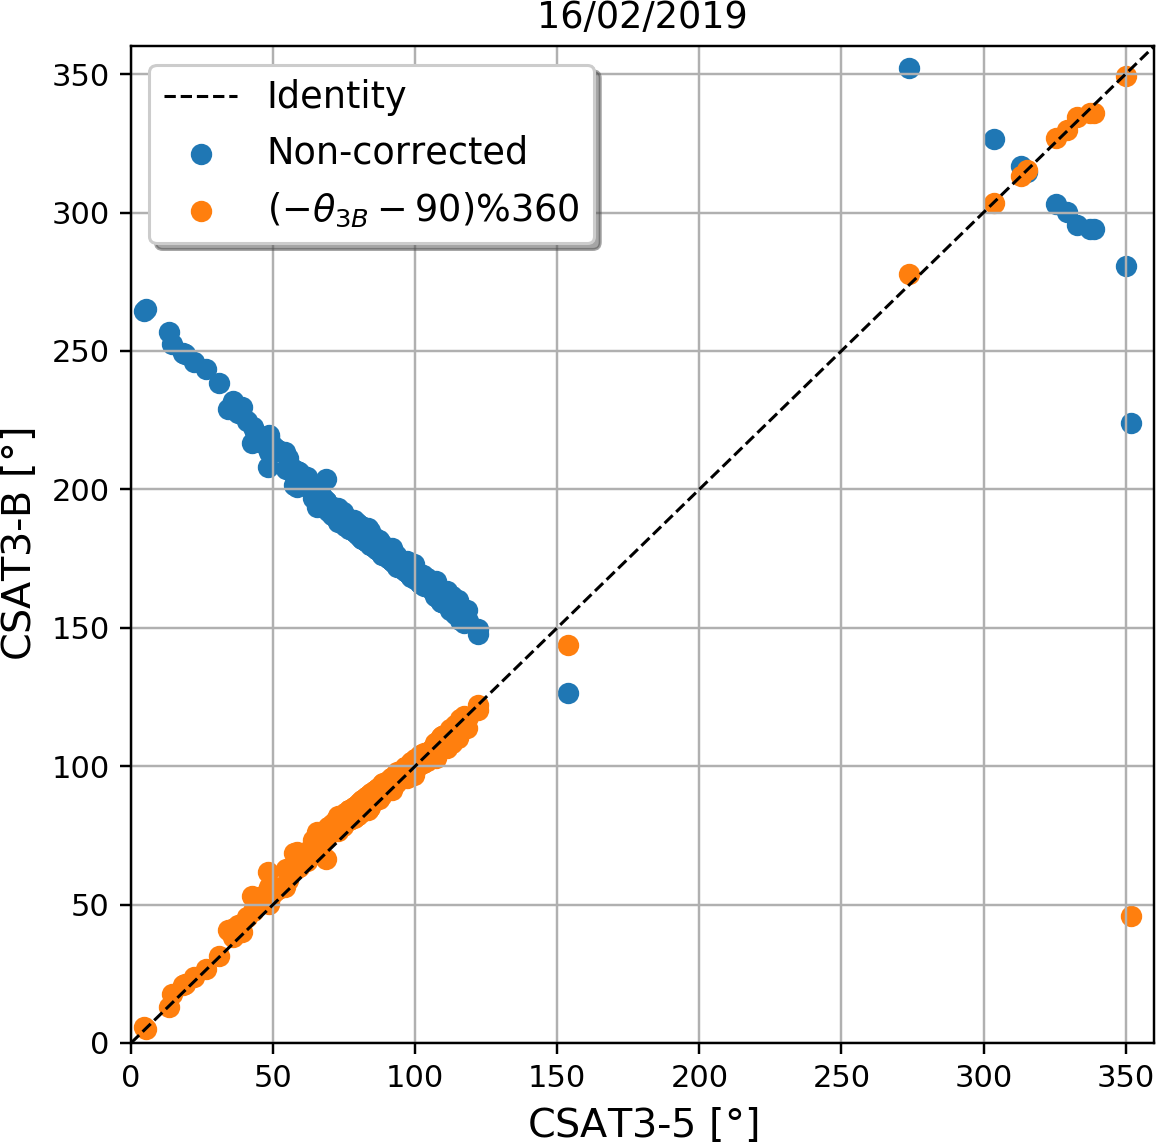
\includegraphics[width=0.48\textwidth]{fig/chapter_4/csat3b_wind_dir.png}
    \caption{Scatter plot comparing the corrected and uncorrected wind direction of the CSAT3-B and the CSAT3 No.5, for the night of the 16th of February.}
    \label{fig:csat3b_correction}
\end{figure}

\section{Vertical profiles of the 16-17th night} \label{app:profiles}

In this section, we present the results of the analysis of the night from the 16th to the 17th of February. In the figure~\ref{fig:16-17_21-23_profiles.png}, we can see the vertical profiles of air temperature and wind speed, with the corresponding wind direction for each time. The data used for these profiles was the 30 minutes averaged data. As we can see in the wind speed profiles, two anemometers were not working during this night, which leaves a gap between 3m and 6m. Despite this detail, is possible to see a wind maximum near the surface, at the level of the CSAT3 No.5 (between 0.5m to 1m).

\begin{figure}[!ht]
    \centering
    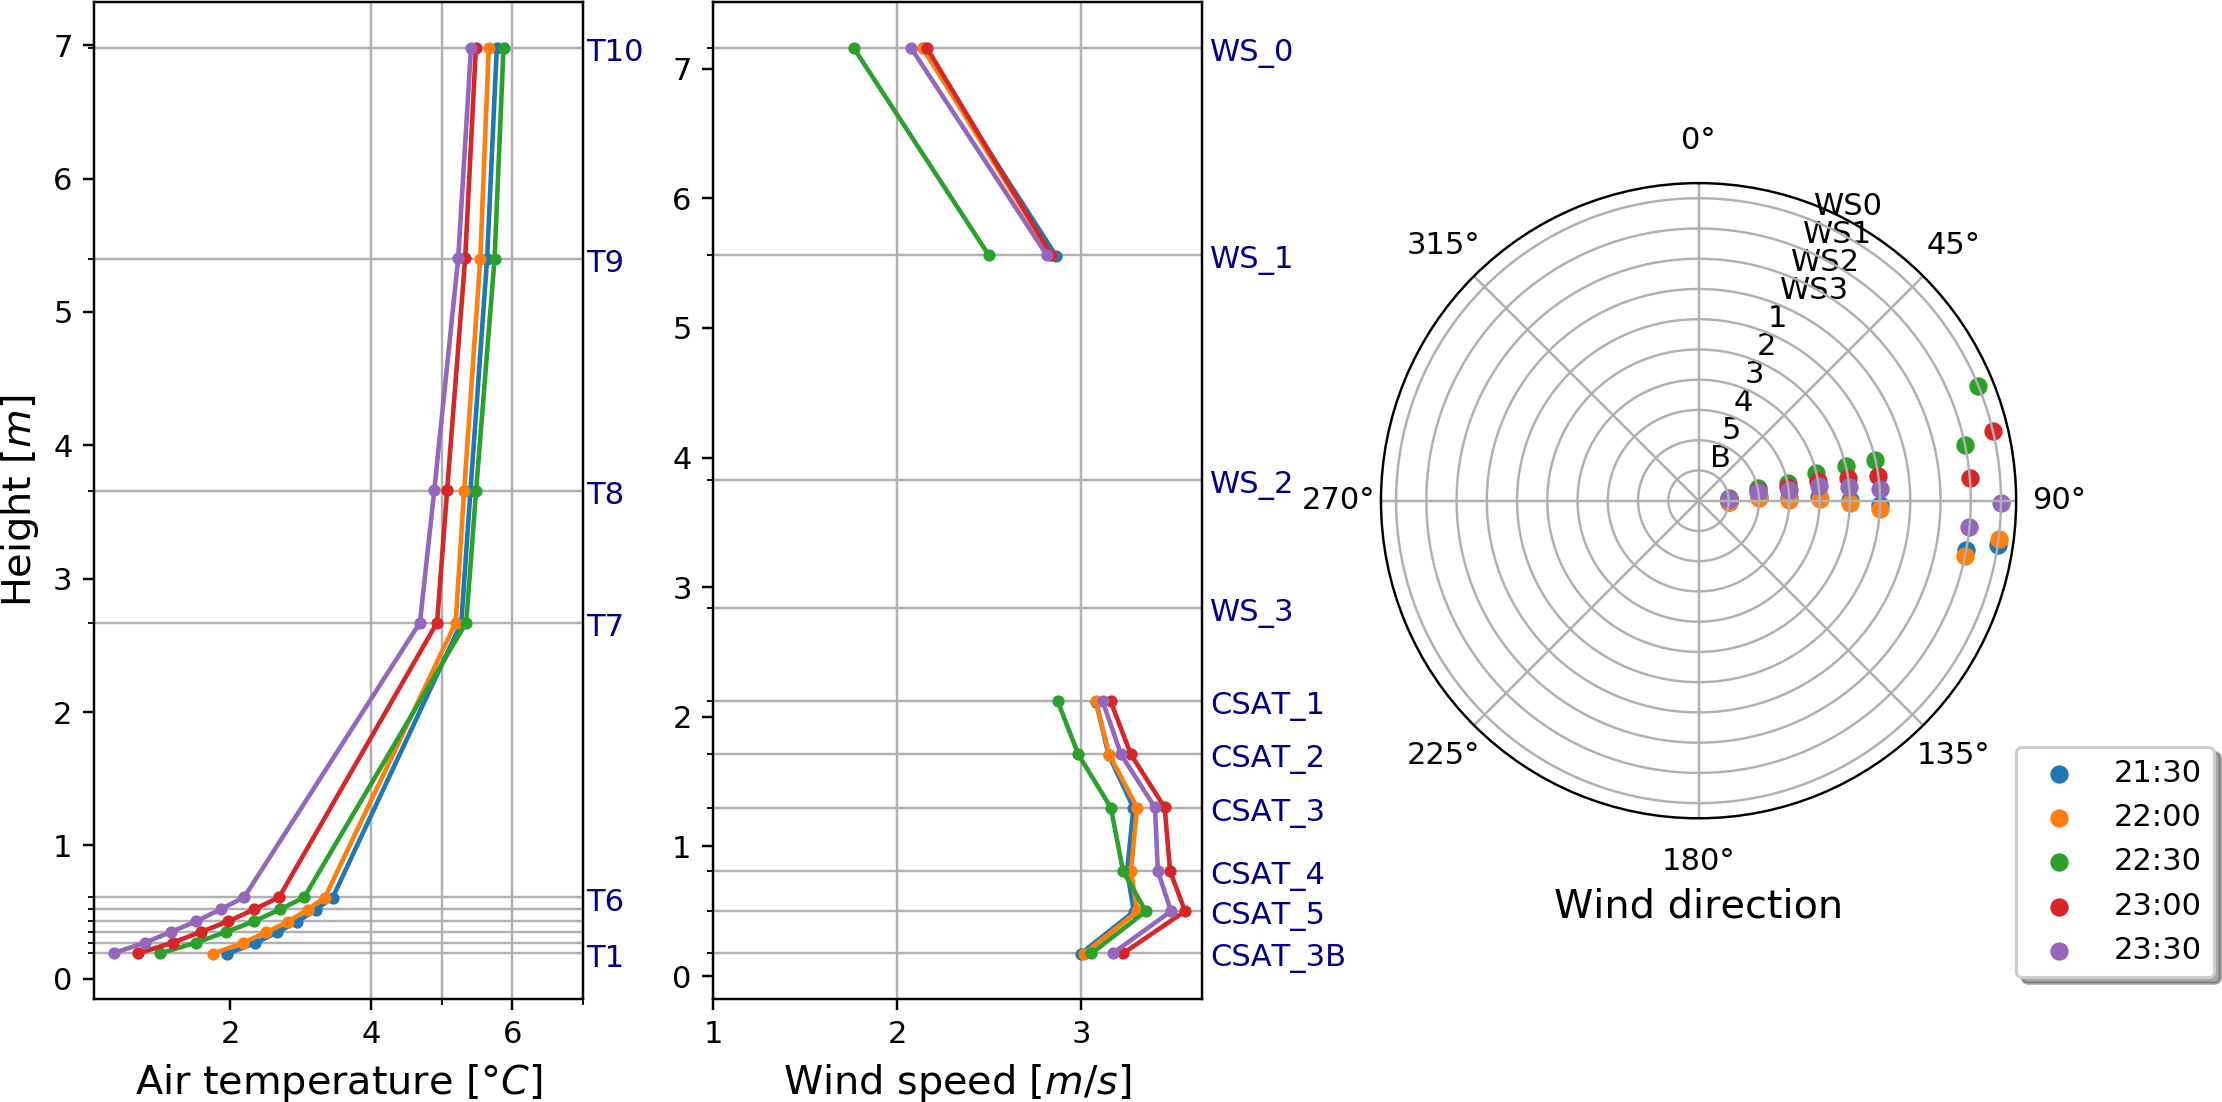
\includegraphics[width=1\textwidth]{fig/chapter_4/16-17/21-23_profiles.png}
    \caption{Temperature and wind speed vertical profiles, with the corresponding wind direction at a particular time, for the period between 21h30 and 23h30 on the night of the 16-17th.}
    \label{fig:16-17_21-23_profiles.png}
\end{figure}

In figure~\ref{fig:16-17_flux_series} we can see the variation of the vertical fluxes $\tau$ and $H$, during the first part of the night. In the bottom part of the figure, we can see the Turbulent Kinetic Energy variation in the same period of time.

\begin{figure}[!ht]
    \centering
    \begin{subfigure}[b]{0.6\textwidth}
        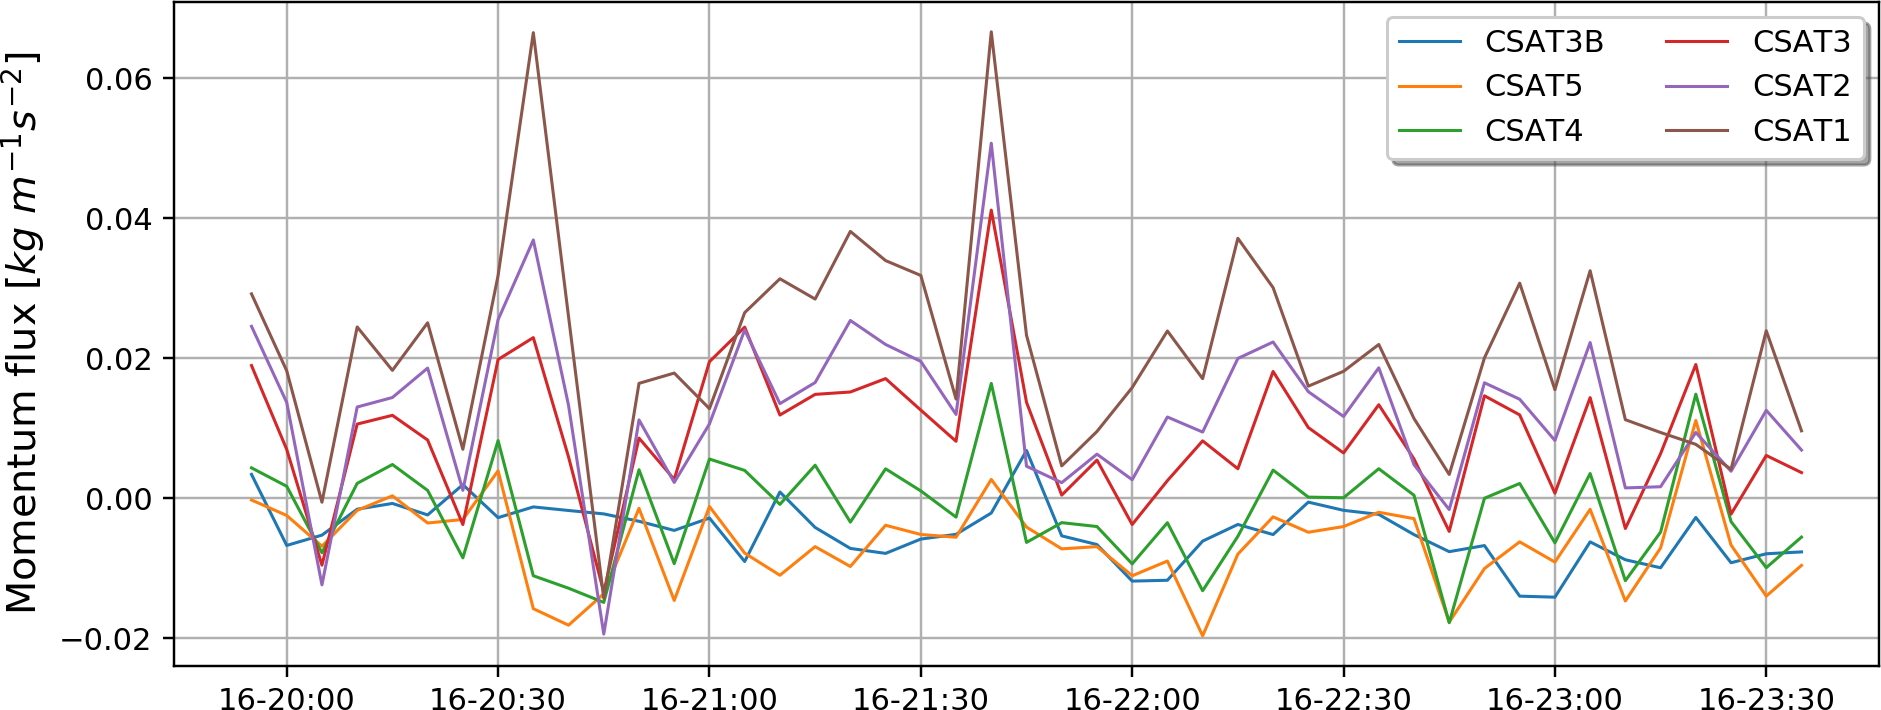
\includegraphics[width=\textwidth]{fig/chapter_4/16-17/Tau_16-17.png}
      \label{fig:Tau_16-17}
    \end{subfigure}
    \begin{subfigure}[b]{0.6\textwidth}
        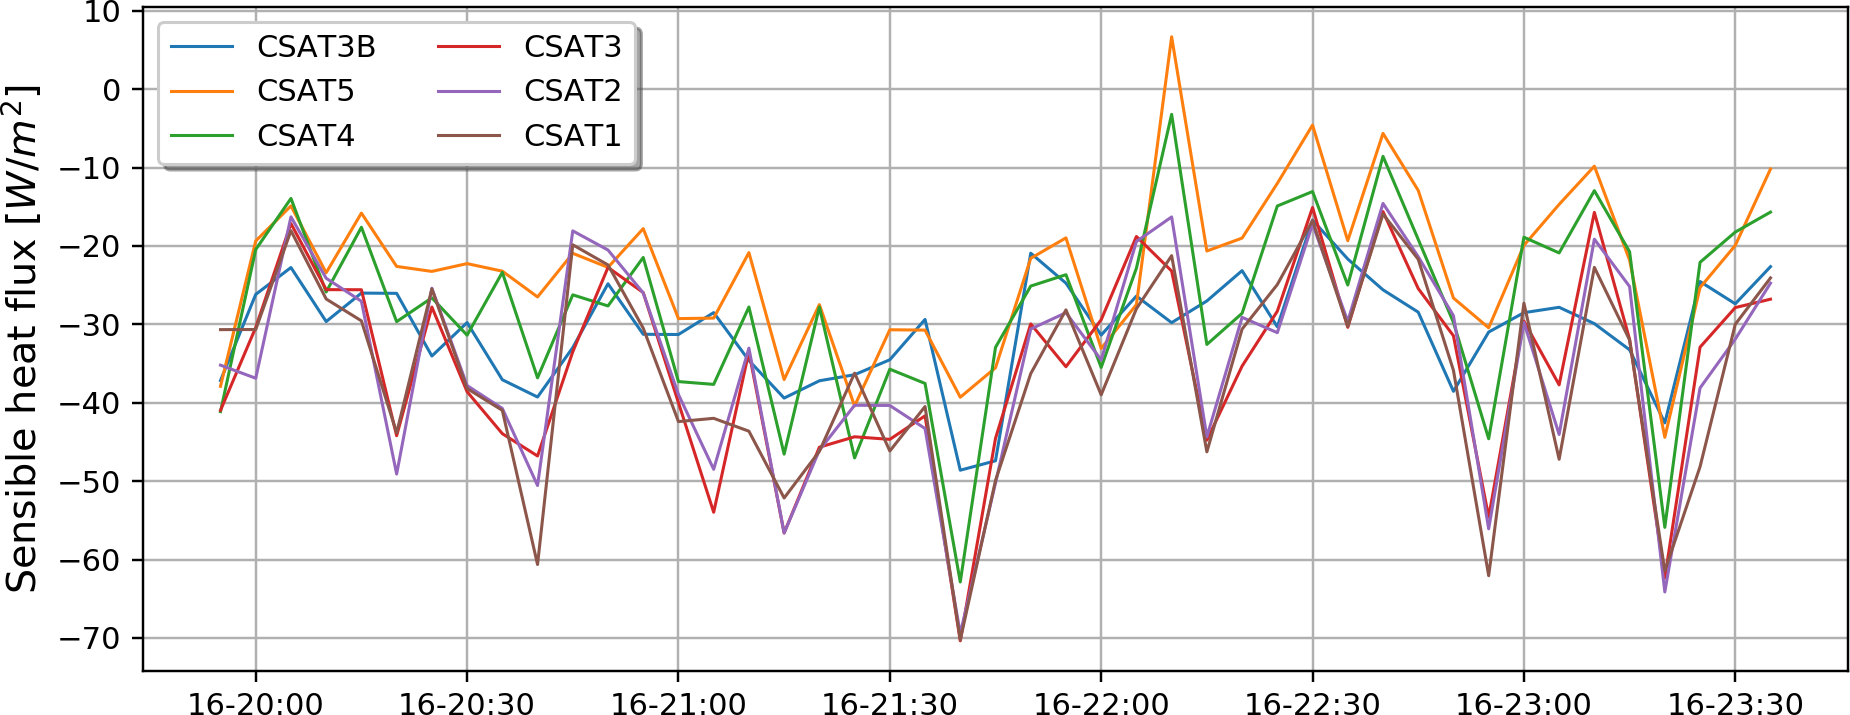
\includegraphics[width=\textwidth]{fig/chapter_4/16-17/H_16-17.png}
        \label{fig:H_16-17}
    \end{subfigure}
    \begin{subfigure}[b]{0.6\textwidth}
        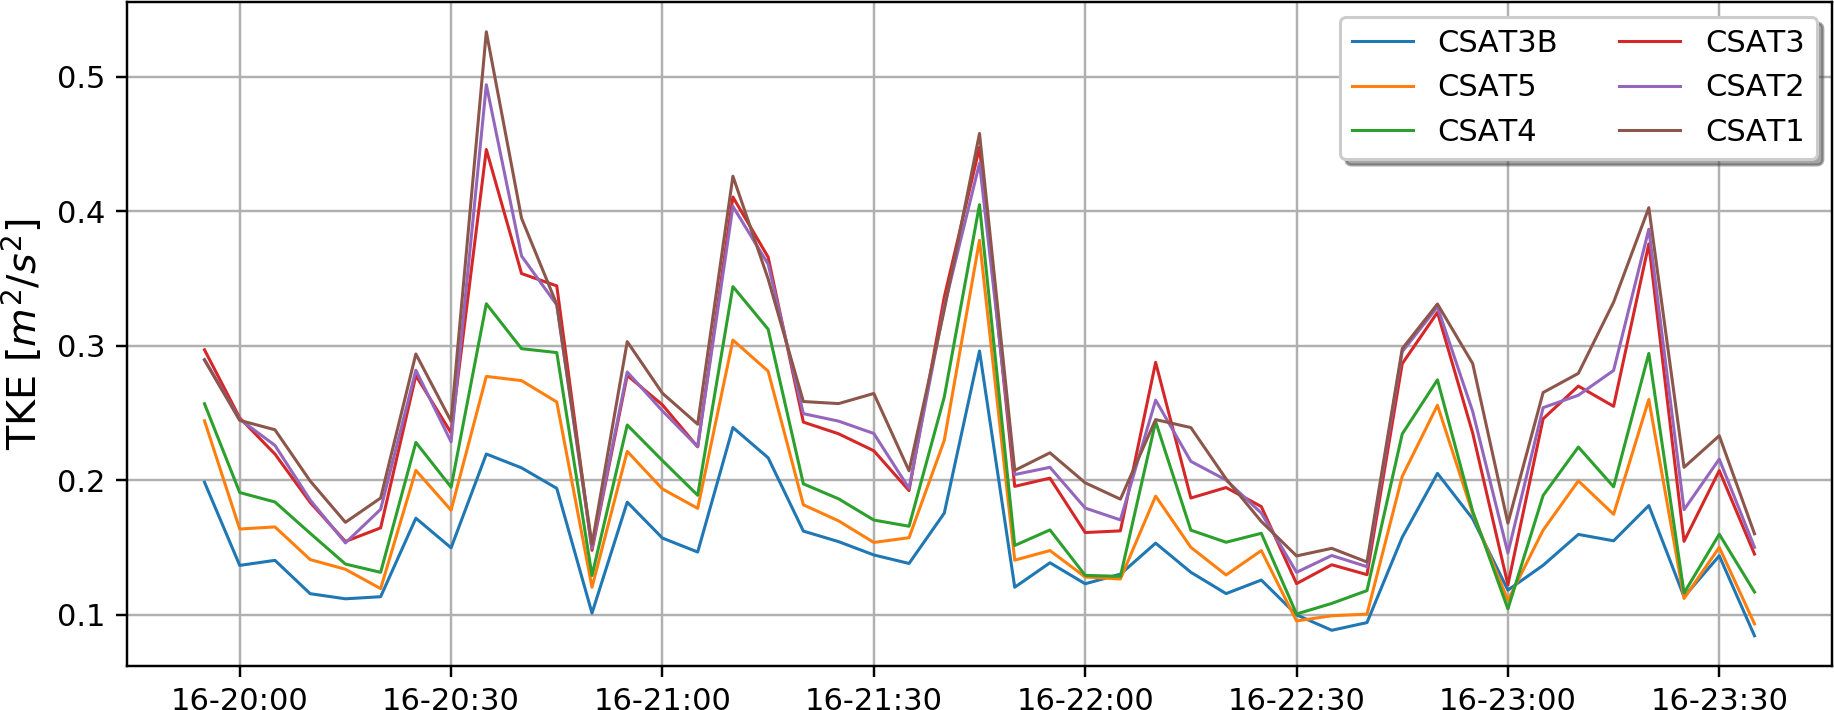
\includegraphics[width=\textwidth]{fig/chapter_4/16-17/TKE_16-17.png}
        \label{fig:TKE_16-17}
    \end{subfigure}
    \caption{Time series of the momentum flux (upper figure), temperature flux (middle figure) and Turbulent Kinetic Energy (lower figure), for the 16-17th night.}
    \label{fig:16-17_flux_series}
\end{figure}

With the help of the profiles of figure~\ref{fig:16-17_21-23_profiles.png}, we selected the data around 23h10, to plot the vertical profiles of the fluxes and the TKE. We can see in the mean wind profiles that the maximum is between 0.5m and 0.75m, except at 23h15 where appears another maximum at 1.25m. Looking at the momentum fluxes, we see that below the maximum $\tau$ is negative, and in theory at the same level of the maximum $\tau = 0$, which is only the case for the 23h05 profile. Looking at the momentum fluxes, we see that all are negative, as in the 23-24th night (see figures \ref{fig:vert_prof_a} and \ref{fig:vert_prof_a}), and there are some variations as we go up. The 23h10 profile shows a fairly constant sensible heat flux except at the lower level of the profile. Finally, for the TKE, we can see that at the lower level it is small, and the TKE increases as the height increases.

\begin{figure}
    \centering
    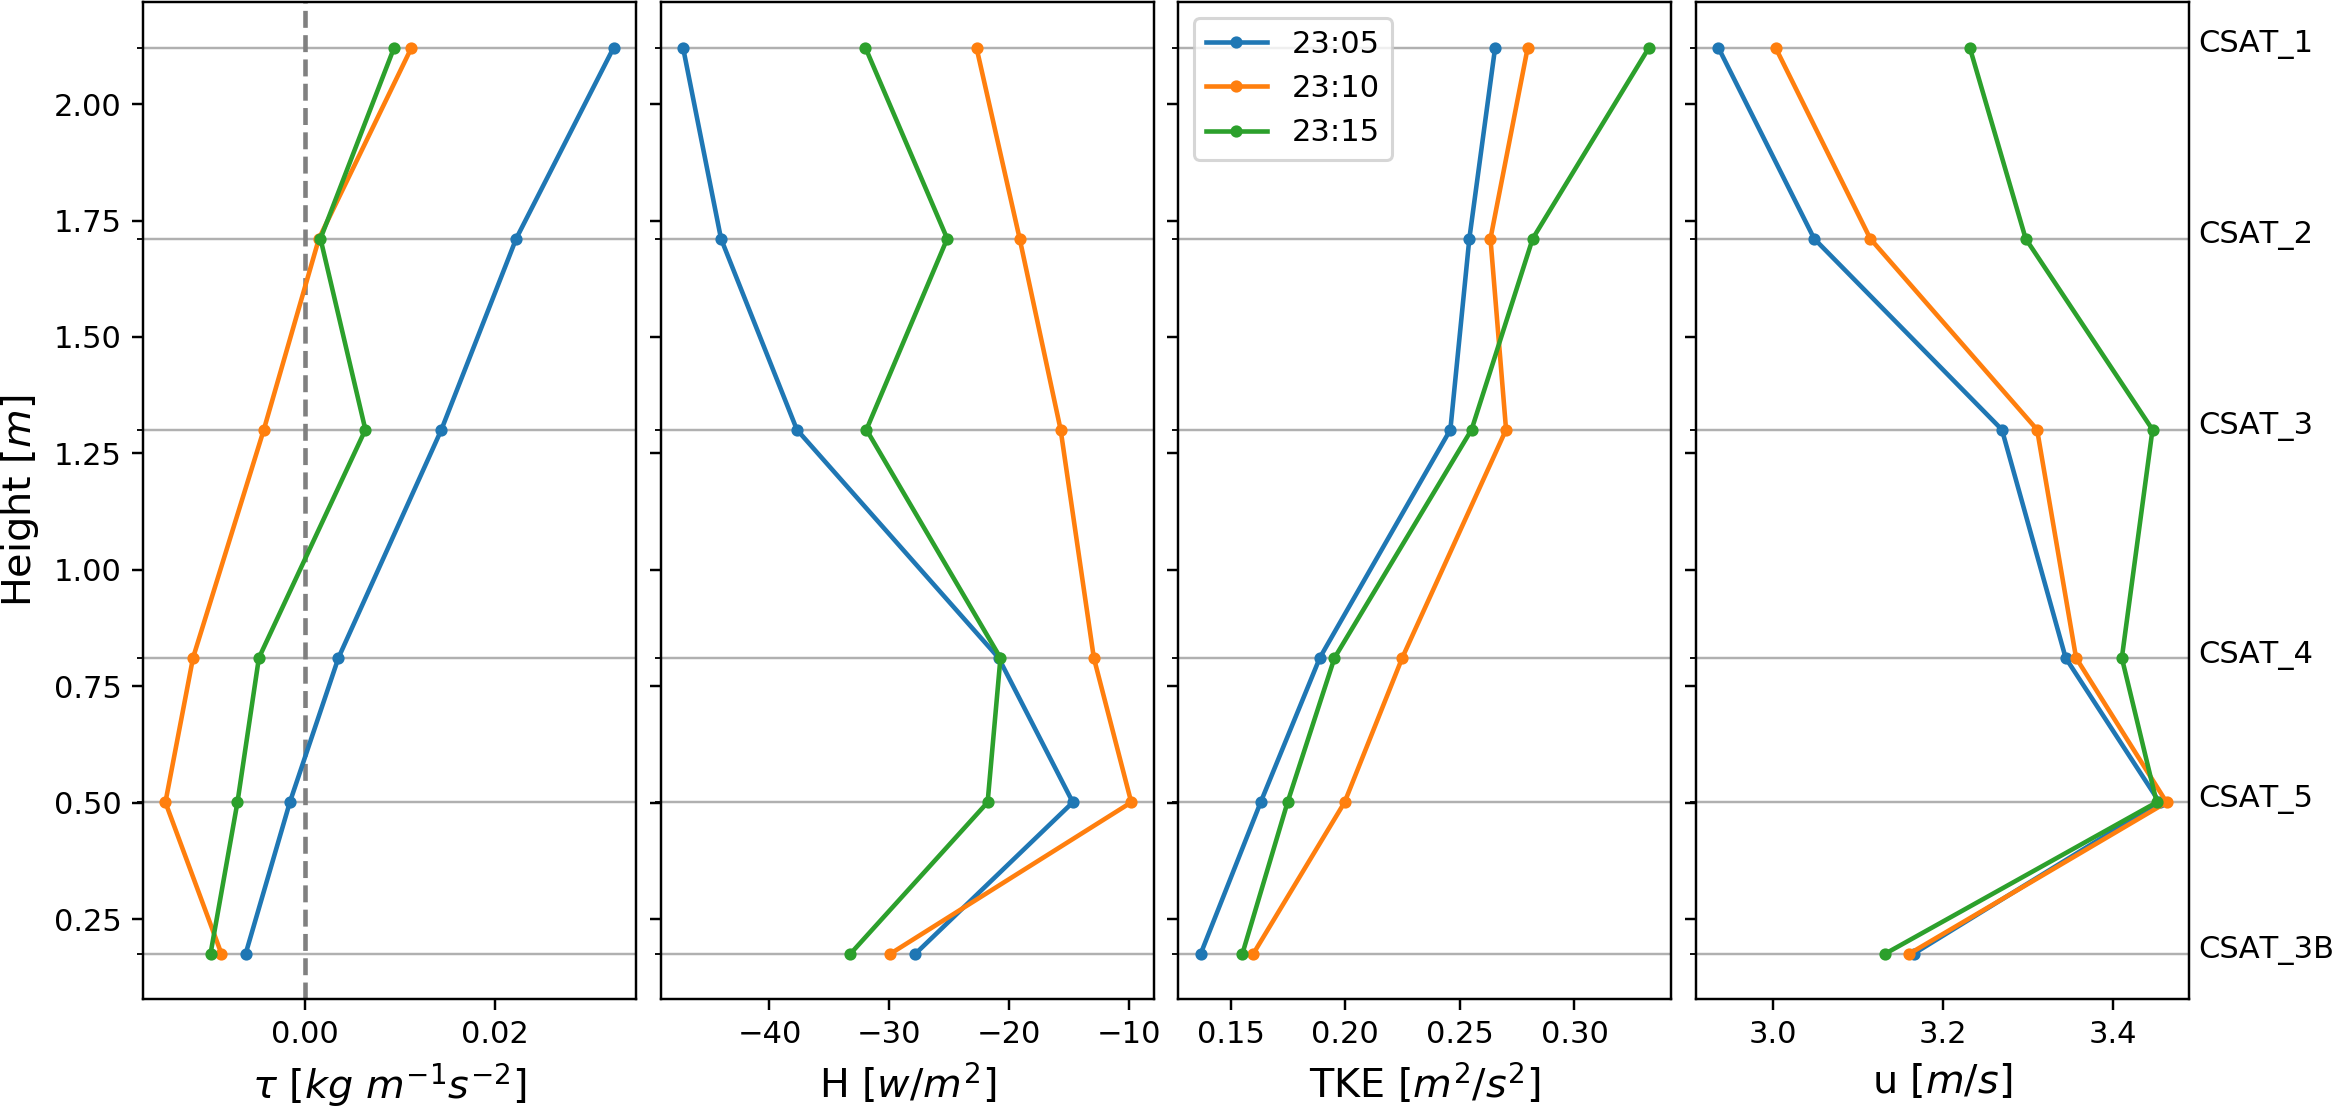
\includegraphics[width=1\textwidth]{fig/chapter_4/16-17/vert_prof_d_speedmax.png}
    \caption{Vertical profiles of momentum flux ($\tau$), sensible heat flux ($H$), Turbulent Kinetic Energy ($TKE$) and wind speed ($u$), for the night of the 16-17th of February, around 23h10.}
    \label{fig:vert_prof_d}
\end{figure}